

%-------------------------------------------------------%
\section{初期値・境界値データの作成:init}
%-------------------------------------------------------%

init では,SCALE計算に必要な初期値・境界値データを作成する.
まず,initディレクトリへ移動する.
\begin{verbatim}
 $ cd scale/scale-les/test/tutorial/init
\end{verbatim}

initディレクトリの中には,\verb|init.conf|という名前のコンフィグファイルが準備されている.
\verb|pp.conf|と同様に,実験設定に合わせて、この\verb|init.conf|を書き換える必要があるが、
チュートリアル用の\verb|init.conf|ファイルはTable\ref{tab:grids}の設定に
すでに合わせてある.
初期値・境界値データの作成には前節で作成した地形・土地利用データを利用する.
これは,下記のように,相対PATHを用いて参照するように設定されている.

\begin{verbatim}
&PARAM_TOPO
 TOPO_IN_BASENAME = "../pp/topo_d01",
/
&PARAM_LANDUSE
 LANDUSE_IN_BASENAME  = "../pp/landuse_d01",
/
\end{verbatim}
その他に\verb|init.conf|の設定の中で特に注意するべき項目は,
\verb|PARAM_MKINIT_REAL|である.

\begin{verbatim}
&PARAM_MKINIT_REAL
 BASENAME_BOUNDARY   = "boundary_d01",  <- 境界値データの出力名
 FILETYPE_ORG        = "NICAM-NETCDF",
 NUMBER_OF_FILES     = 2,               <- 読み込むファイルの数
 BOUNDARY_UPDATE_DT  = 21600.D0,        <- 入力データの時間間隔
 INTERP_SERC_DIV_NUM = 20,              <- 内挿計算用のチューニングパラメータ
/
\end{verbatim}

\verb|FILETYPE_ORG|は入力する気象場データのファイルフォーマットに
関するパラメータを設定しており,ここでは
NICAMモデルのnetcdf形式データのフォーマットで読み込むことを指定している.
詳細なコンフィグファイルの内容については,Appendix \ref{app:namelist}を参照されたい.

次に,コンパイル済みのバイナリをinitディレクトリへリンクする.
\begin{verbatim}
 $ ln -s ${TOPDIR}/bin/scale-les_init ./
\end{verbatim}
入力データはinitディレクトリの中に準備されている,\verb|"inputdata-link.sh"|を用いてリンクする.
\begin{verbatim}
 $ sh inputdata-link.sh
\end{verbatim}
としてスクリプトを実行することで,気象場の入力データがリンクされ,initディレクトリ内に下記のファイルがリンクされる.
このスクリプトにあるstart dateとend dateの設定項目を実験設定に対応するように編集するが、ここでは,start dateは1999/05/05 00:00:00,end dateは1999/05/06 00:00:00と設定している.もし,\verb|tutorial_data|を\verb|${TOPDIR}/data|以外の場所に展開している場合は,スクリプト内の
\verb|"dir"|の項目も適切なディレクトリに変更すること.下記ファイルにリンクが張れれば成功.
{\small
\begin{verbatim}

la_tg_00000.peall.nc    ms_qv_00000.peall.nc   oa_sst_00000.peall.nc  ss_tem_sfc_00000.peall.nc
la_tg_00001.peall.nc    ms_qv_00001.peall.nc   oa_sst_00001.peall.nc  ss_tem_sfc_00001.peall.nc
la_wg_00000.peall.nc    ms_tem_00000.peall.nc  ss_q2m_00000.peall.nc  ss_u10m_00000.peall.nc
la_wg_00001.peall.nc    ms_tem_00001.peall.nc  ss_q2m_00001.peall.nc  ss_u10m_00001.peall.nc
lsmask_00000.peall.nc   ms_u_00000.peall.nc    ss_slp_00000.peall.nc  ss_v10m_00000.peall.nc
lsmask_00001.peall.nc   ms_u_00001.peall.nc    ss_slp_00001.peall.nc  ss_v10m_00001.peall.nc
ms_pres_00000.peall.nc  ms_v_00000.peall.nc    ss_t2m_00000.peall.nc
ms_pres_00001.peall.nc  ms_v_00001.peall.nc    ss_t2m_00001.peall.nc

\end{verbatim} }

次に、陸面過程や放射過程のモデルを起動するためのパラメータファイルにリンクをはる.
\begin{verbatim}
 $ ln -s scale/scale-les/test/data/land/*  ./
 $ ln -s scale/scale-les/test/data/rad/*   ./
\end{verbatim}
上の行のリンクコマンドによって陸面過程のパラメータファイルがリンクされ,
下の行のコマンドによって放射過程のパラメータファイルがリンクされる.
準備が整ったら,9つのMPIプロセスを使用してinitを実行する.
\begin{verbatim}
 $ mpirun -n 9 ./scale-les_init init.conf
\end{verbatim}

正常にジョブが終了すれば,
\verb|boundary_d01.pe######.nc|と\verb|init_d01_00010713600.000.pe######.nc|というファイルが
MPIプロセス数だけ,つまり9つずつ生成される(\verb|######|にはMPIプロセスの番号が入る).
それぞれ,境界値データと初期値データが入ってるおり,境界値データには複数の時刻のデータが1つのファイルに含まれている.
初期値ファイルの名前のうち\verb|"00010713600.000"|の部分は,モデル内で算出された実験開始時刻を表している.

処理内容のログとして,\verb|init_LOG_d01.pe000000|という名前でログファイルも出力されるので内容を確かめておくこと.
gpviewがインストールされていれば,次のコマンドによって作成された地形と土地利用データを描画してチェックすることができる.
正しく作成されていれば,Fig. \ref{fig:init}と同じように描かれる.

\begin{verbatim}
$ gpvect --scalar --slice z=1500 --nocont --aspect=1 --range=0.001:0.015          \
         --xintv=10 --yintv=10 --unit_vect init_d01_00010713600.000.pe00*@QV      \
         init_d01_00010713600.000.pe00*@MOMX init_d01_00010713600.000.pe00*@MOMY
\end{verbatim}


\begin{figure}[h]
\begin{center}
  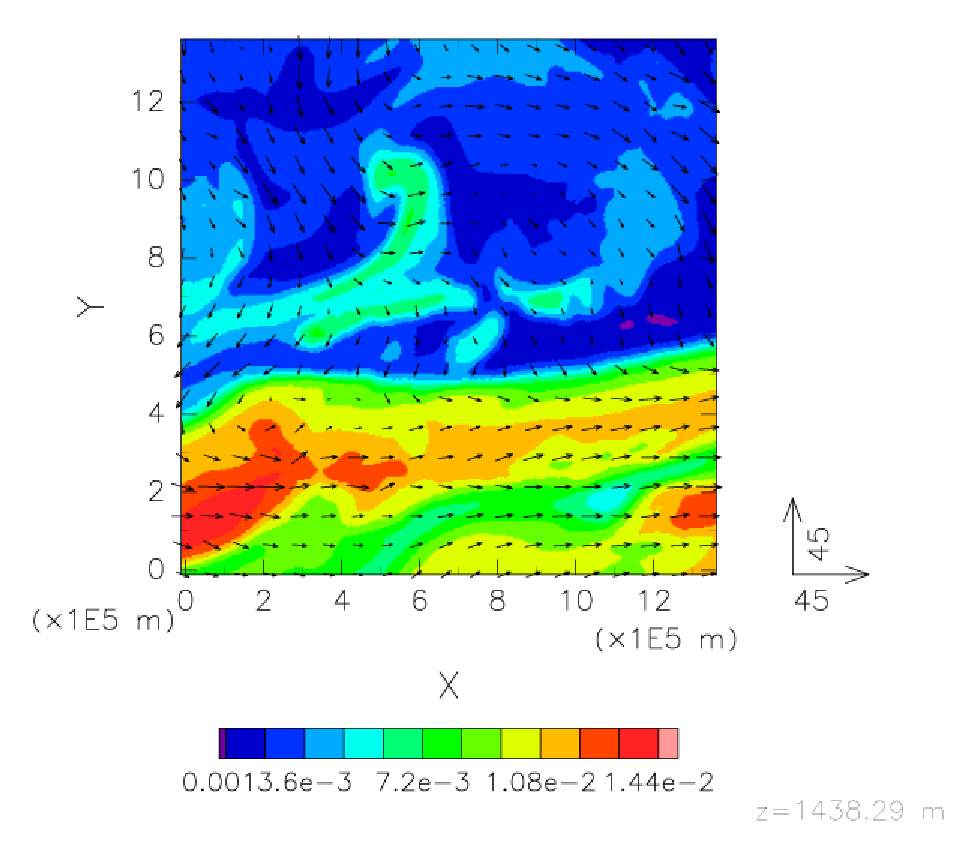
\includegraphics[width=0.7\hsize]{./figure/init_qv-momxy.eps}\\
  \caption{チュートリアル実験の初期場の様子:カラーシェードは高度1.5kmにおける比湿の分布,ベクトルは高度1.5kmにおける水平運動量フラックスを表している.}
  \label{fig:init}
\end{center}
\end{figure}


